\chapter[Gerenciamento de requisitos]{Gerenciamento de requisitos}
\section{Atributos de um requisito}
Os atributos contém as informações mais importantes daquele requisito, são suas propriedades, e é a partir dessas propriedades que se tem informações como: data de criação, origem, importância, dentre outras. Demandam atenção durante a sua especificação, pois fornecem importantes informações sobre o estado do projeto, além de permitirem que sejam realizadas consultas dentro de todos os requisitos.
Os atributos definidos para gerenciar os requisitos durante a execução do nosso projeto foram:
  \begin{figure}[!htbp]
    \centering
    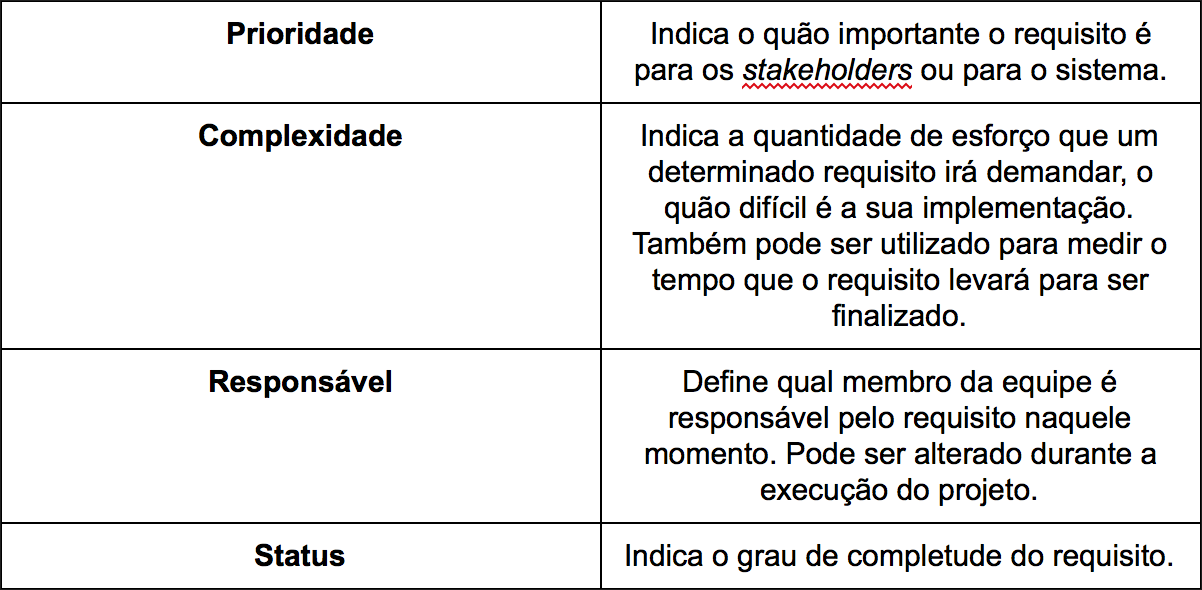
\includegraphics[scale=0.5]{editaveis/figuras/tabela_atributos}
    \caption[Atributos dos requisitos do projeto]{Atributos dos requisitos do projeto. \footnotemark}
    \label{tabela_atributos}
  \end{figure}
\subsection{Prioridade}
\begin{itemize}
\item \textbf{Alta} - Indica vital importância para o sistema e para os stakeholders, normalmente agrega um grande valor aos usuários.
\item \textbf{Média} - Indica relativa importância para o sistema e para os stakeholders, normalmente são requisitos que não foram compreendidos em sua totalidade pela equipe e podem ser implementados quando o cliente achar necessário.
\item \textbf{Baixa} - Indica uma baixa importância para o sistema e para os stakeholders, normalmente representam funcionalidades opcionais para a realização do sistema.
\end{itemize}
\subsection{Complexidade}
\begin{itemize}
\item \textbf{Alta} - Indica alto nível de dificuldade, demandando um alto nível de esforço para a sua implementação.
\item \textbf{Média} - Indica um relativo nível de dificuldade, demandando um moderado nível de esforço para a sua implementação.
\item \textbf{Baixa} - Indica um baixo nível de dificuldade, demandando um baixo nível de esforço para a sua implementação.
\end{itemize}
\subsection{Responsável}
Identifica na equipe o membro responsável pelo requisito naquele momento.
\subsection{Status}
\begin{itemize}
\item \textbf{Finalizado} - Indica a realização daquele requisito e sua implementação no sistema.
\item \textbf{Em progresso} - Indica que o requisito está sendo implementado no sistema.
\item \textbf{Não iniciado} - Indica que o processo de implementação daquele requisito não teve início.
\end{itemize}
\section{Rastreabilidade de requisitos}
Rastreabilidade de software é a habilidade de relacionar artefatos criados durante o ciclo de vida de desenvolvimento de um sistema de software.[1] Os elementos rastreáveis do projeto são chamados de itens de rastreabilidade.
O rastreamento de requisitos pode ser visto como uma habilidade de acompanhar e descrever a vida de um requisito em abas as direções. A pré-rastreabilidade documenta o contexto a partir do qual emergem os requisitos, já a pós-rastreabilidade vincula os requisitos ao desenho do sistema e sua implementação.(DAVIS, 1993).
(FINALIZAR)
\section{Gestão de requisitos}